\documentclass[2pt,a4paper]{article}
\usepackage{fontspec, xunicode, xltxtra}
\XeTeXlinebreaklocale "zh"
\XeTeXlinebreakskip = 0pt plus 1pt minus 0.1pt
\setmainfont{SimSun}
\title{PI2}
\begin{document}
\author{Evangelos A.Theodorou}
\section{带有路径积分的随机梯度下降}
\subsection{随机最优控制的定义和符号}
对于我们的技术发展,我们将使用来自路径最优控制领域的控制信息记号,然而,由于我们试图有和标准RL记号尽可能多的交叠,我们对于一个路径$\tau_i$定义一个有限长度的代价函数,在时刻$\t_i$,状态$x_{t_i}$开始,在时刻$t_N$结束,\\
$R(t_i)=\phi_{t_N}+\int _{t_i} ^{t_N} r_tdt$\\
$\phi_{t_N}=\phi(x_{t_N})$代表时刻$t_N$的终止奖励,$r_t$代表时刻$t$的即刻代价。在随机最优控制领域,目标是找到控制动作$u_t$能够最小化值函数。\\
我们考虑一般的控制系统:\\
$\dot{x}_t=f(x_t,t)+G(x_t)(u_t+\epsilon_t)=f_t+G_t(u_t+\epsilon_t)$\\
$x_t$系统状态,$G_t$控制矩阵,$f_t$被动dynamics,$u_t$控制向量,$\epsilon_t$高斯噪声,带有方差$\Sigma_{\epsilon}$,考虑下列代价函数:\\
$r_t=r(x_t,u_t,t)=q_t+\frac{1}{2}u_t^TRu_t$\\
$q_t=q(x_t,t)$任意的状态独立的代价函数,$R$半正定权重矩阵和均方控制代价。随机的HJB等式将表示如下:\\
$\partial_tV_t=\mathop{min}\limits_{u}(r_t+(\Delta_xV_t)^TF_t+\frac{1}{2}trace((\Delta_{xx}V_t)G_t\Sigma_{\epsilon}G_t^T))$\\
$F_t=f(x_t,t)+G(x_t)u_t$,为了找到最小值,代价函数插入到上式,圆括号\footnote{parentesis,圆括号,插入语,间歇}内的表达式的梯度是关于$u$的,并且设为0。相关的最优化控制信号通过下面的等式给出:\\
$u(x_t)=u_t=-R^{-1}G_t^T(\Delta_{x_t}V_t)$\\
把上面的最优化控制代入\footnote{substitution,代替;置换;代替物}HJB,得到下面的非线性二阶偏微分等式(PDE):\\
$\partial_tV_t=q_t+(\Delta_xV_t)^Tf_t-\frac{1}{2}(\Delta_xV_t)^TG_tR^{-1}G_t^T(\Delta_xV_t)+\frac{1}{2}trace((\Delta_{xx}V_t)G_t\Sigma_{\epsilon}G_t^T)$\\
$\Delta_x,\Delta_{xx}$符号分别指的是状态x的雅克比和海森矩阵,$\partial_t$是对时间的偏导数。为了简写,我们经常用下标符号代表时间和状态依赖。
\subsection{将HJB转化为线性PDE}
为了找到上述PDE的解,我们使用值函数的指数变换:\\
$V_t=-\lambda \mathbf{log} \Phi_t$\\
在给出对数变换的情况下,值函数对于时间和状态的偏导数可以写成如下形式:\\
$\partial_t V_t=-\lambda \frac{1}{\Phi_t}\partial_t\Phi_t$\\
$\Delta_x V_t=-\lambda \frac{1}{\Phi_t} \partial_x \Phi_t$\\
$\Delta_{xx}V_t=\lambda \frac{1}{\phi_t^2} \Delta_x \Phi_t \Delta_x \Phi_t^T-\lambda \frac{1}{\Phi_t}\Delta_{xx}\Phi_t$
插入PDE可得,\\
$\frac{\lambda}{\Phi_t}\partial_t \phi_t = q_t -\frac{\lambda}{\Phi_t}(\Delta_x \Phi_t)^Tf_t-\frac{\lambda^2}{2\Phi_t^2}(\Delta_x \Phi_t)^T G_t R^{-1}G_t^T(\Delta_x \Phi_t)+\frac{1}{2}trace(\Gamma) (6)$\\
其中,$\Gamma=(\lambda \frac{1}{\Phi_t^2}\Delta_x \Phi_t \Delta_x \Phi_t^T -\lambda \frac{1}{\Phi_t}\Delta_{xx}\Phi_t)G_t\Sigma_{\epsilon}G_t^T$\\
因此,$\Gamma$的迹是:\\
$trace(\Gamma)=\lambda \frac{1}{\Phi^2}trace (\Delta_x \Phi_t^TG_t\Sigma_{\epsilon}G_t\Delta_x \Phi_t)-\lambda \frac{1}{\Phi_t}trace(\Delta_{xx}\Phi_tG_t\Sigma_{\epsilon}G_t^T)$\\
比较划线的项,可以发现这些项可以取消,如果在$\lambda R^{-1}=\Sigma_{\epsilon}$的假设下,可以有下面的简化:\\
$\lambda G_t R^{-1}G_t^T=G_t\Sigma_{\epsilon}G_t^T=\Sigma(x_t)=\Sigma_t$\\
这个假设背后的直觉是,因为权重控制矩阵和噪声的方差成反比,一个高方差控制输入暗示着廉价的控制代价,反之亦然。从控制论的立场看,这样的关系是有道理的,因为在大干扰(等价于高方差)显著的控制权威要求将系统带到一个想要的状态。这个控制权威可以通过相应的R的低控制输出实现。\\
带着这个简化,(6)可以化简为:\\
$-\partial_t \Phi_t= -\frac{1}{\lambda}q_t\Phi_t+f_t^T(\Delta_x \Phi_t)+\frac{1}{2}trace((\Delta_{xx}\Phi_t)G_t\Sigma_{\epsilon}G_t^T)(9)$\\
在边界条件下:$\Phi_{t_N}=exp(-\frac{1}{\lambda}\phi_{t_N})$.PDE和所谓的Chapman Kolmogorov PDE相关,二阶,线性。在一般情况下,对于一般的非线性系统和代价函数,对于(9)式不能找到分析性解法。然而,PDE的解和它们作为随机微分方程(SDE)的表示有联系,在数学上是通过Feynman-Kac公式表示的。Feynman-Kac公式可以被用来找到随机过程的分布,对于解决特定的SDE和提出很多解决特定SDE的方法。应用这个定理,(9)式可以写成:\\
$\Phi_{t_i}=E_{\tau_i}(\Phi_{t_N}e^{-\int _{t_i}^{t_N} \frac{1}{\lambda} q_t \mathbf{d}t})=E_{\tau_i}[exp(-\frac{1}{\lambda}\phi_{t_N}-\frac{1}{\lambda} \int _{t_i} ^{t_N}q_t dt)] (10)$\\
因此,我们已经把我们的随机最优控制问题转化成了路径积分的近似问题。带着离散时间近似的观点,为数字实现所需的,(10)的解可以写作:\\
$\Phi_{t_i}=\mathop{lim}\limits_{dt \rightarrow 0} \int p(\tau_i|x_i)exp[-\frac{1}{\lambda}(\phi_{t_N}+\sum _{j=i}^{N-1}q_{t_j}dt)]d \tau_i$\\
这里$\tau_i$是从状态$x_{t_i}$开始的采样路径,$p(\tau_i|x_i)$是在起始状态$x_{t_i}$条件下的采样路径的概率。因为(11)式提供了在状态$x_{t_i}$处的指数代价$\Phi_{t_i}$,上面的集成是关于采样路径的。微分项被定义为$d\tau_i=(dx_{t_i},...,dx_{t_N})$.(11)式的随机积分的评估要求具体指出$p(\tau_i|x_i)$,这正式下一节我们所讨论的问题。
\subsection{一般的路径积分等式}
为了形成我们的算法,我们需要考虑比Kappen和Broek提出的随机最优控制更加普遍的路径积分方法。尤其是,我们必须指出,在很多随机动态系统中,控制转移矩阵$G_t$是状态独立的,因此它的结构依赖于状态的直接部分和不直接激活的部分。因为仅仅一些状态是直接控制的,状态向量可以拆分成$x=[x^{(m)^T} \quad x^{(c)^T}]^T$.紧接着,被动的动力学项和控制转移矩阵可以拆分成$x=[f_t^{(m)^T} \quad f_t^{(c)^T}]^T$,$G_t=[0_{k*p} \quad G_t^{(c)^T}]^T$\\
这种系统的离散的状态空间表示如下:\\
$x_{t_{i+1}}=x{t_i}+f_{t_i}dt+G_{t_i}(u_{t_i}dt+\sqrt{dt}\epsilon_{t_i})$\\
\begin{figure}
    		   \centering
  		   \centerline{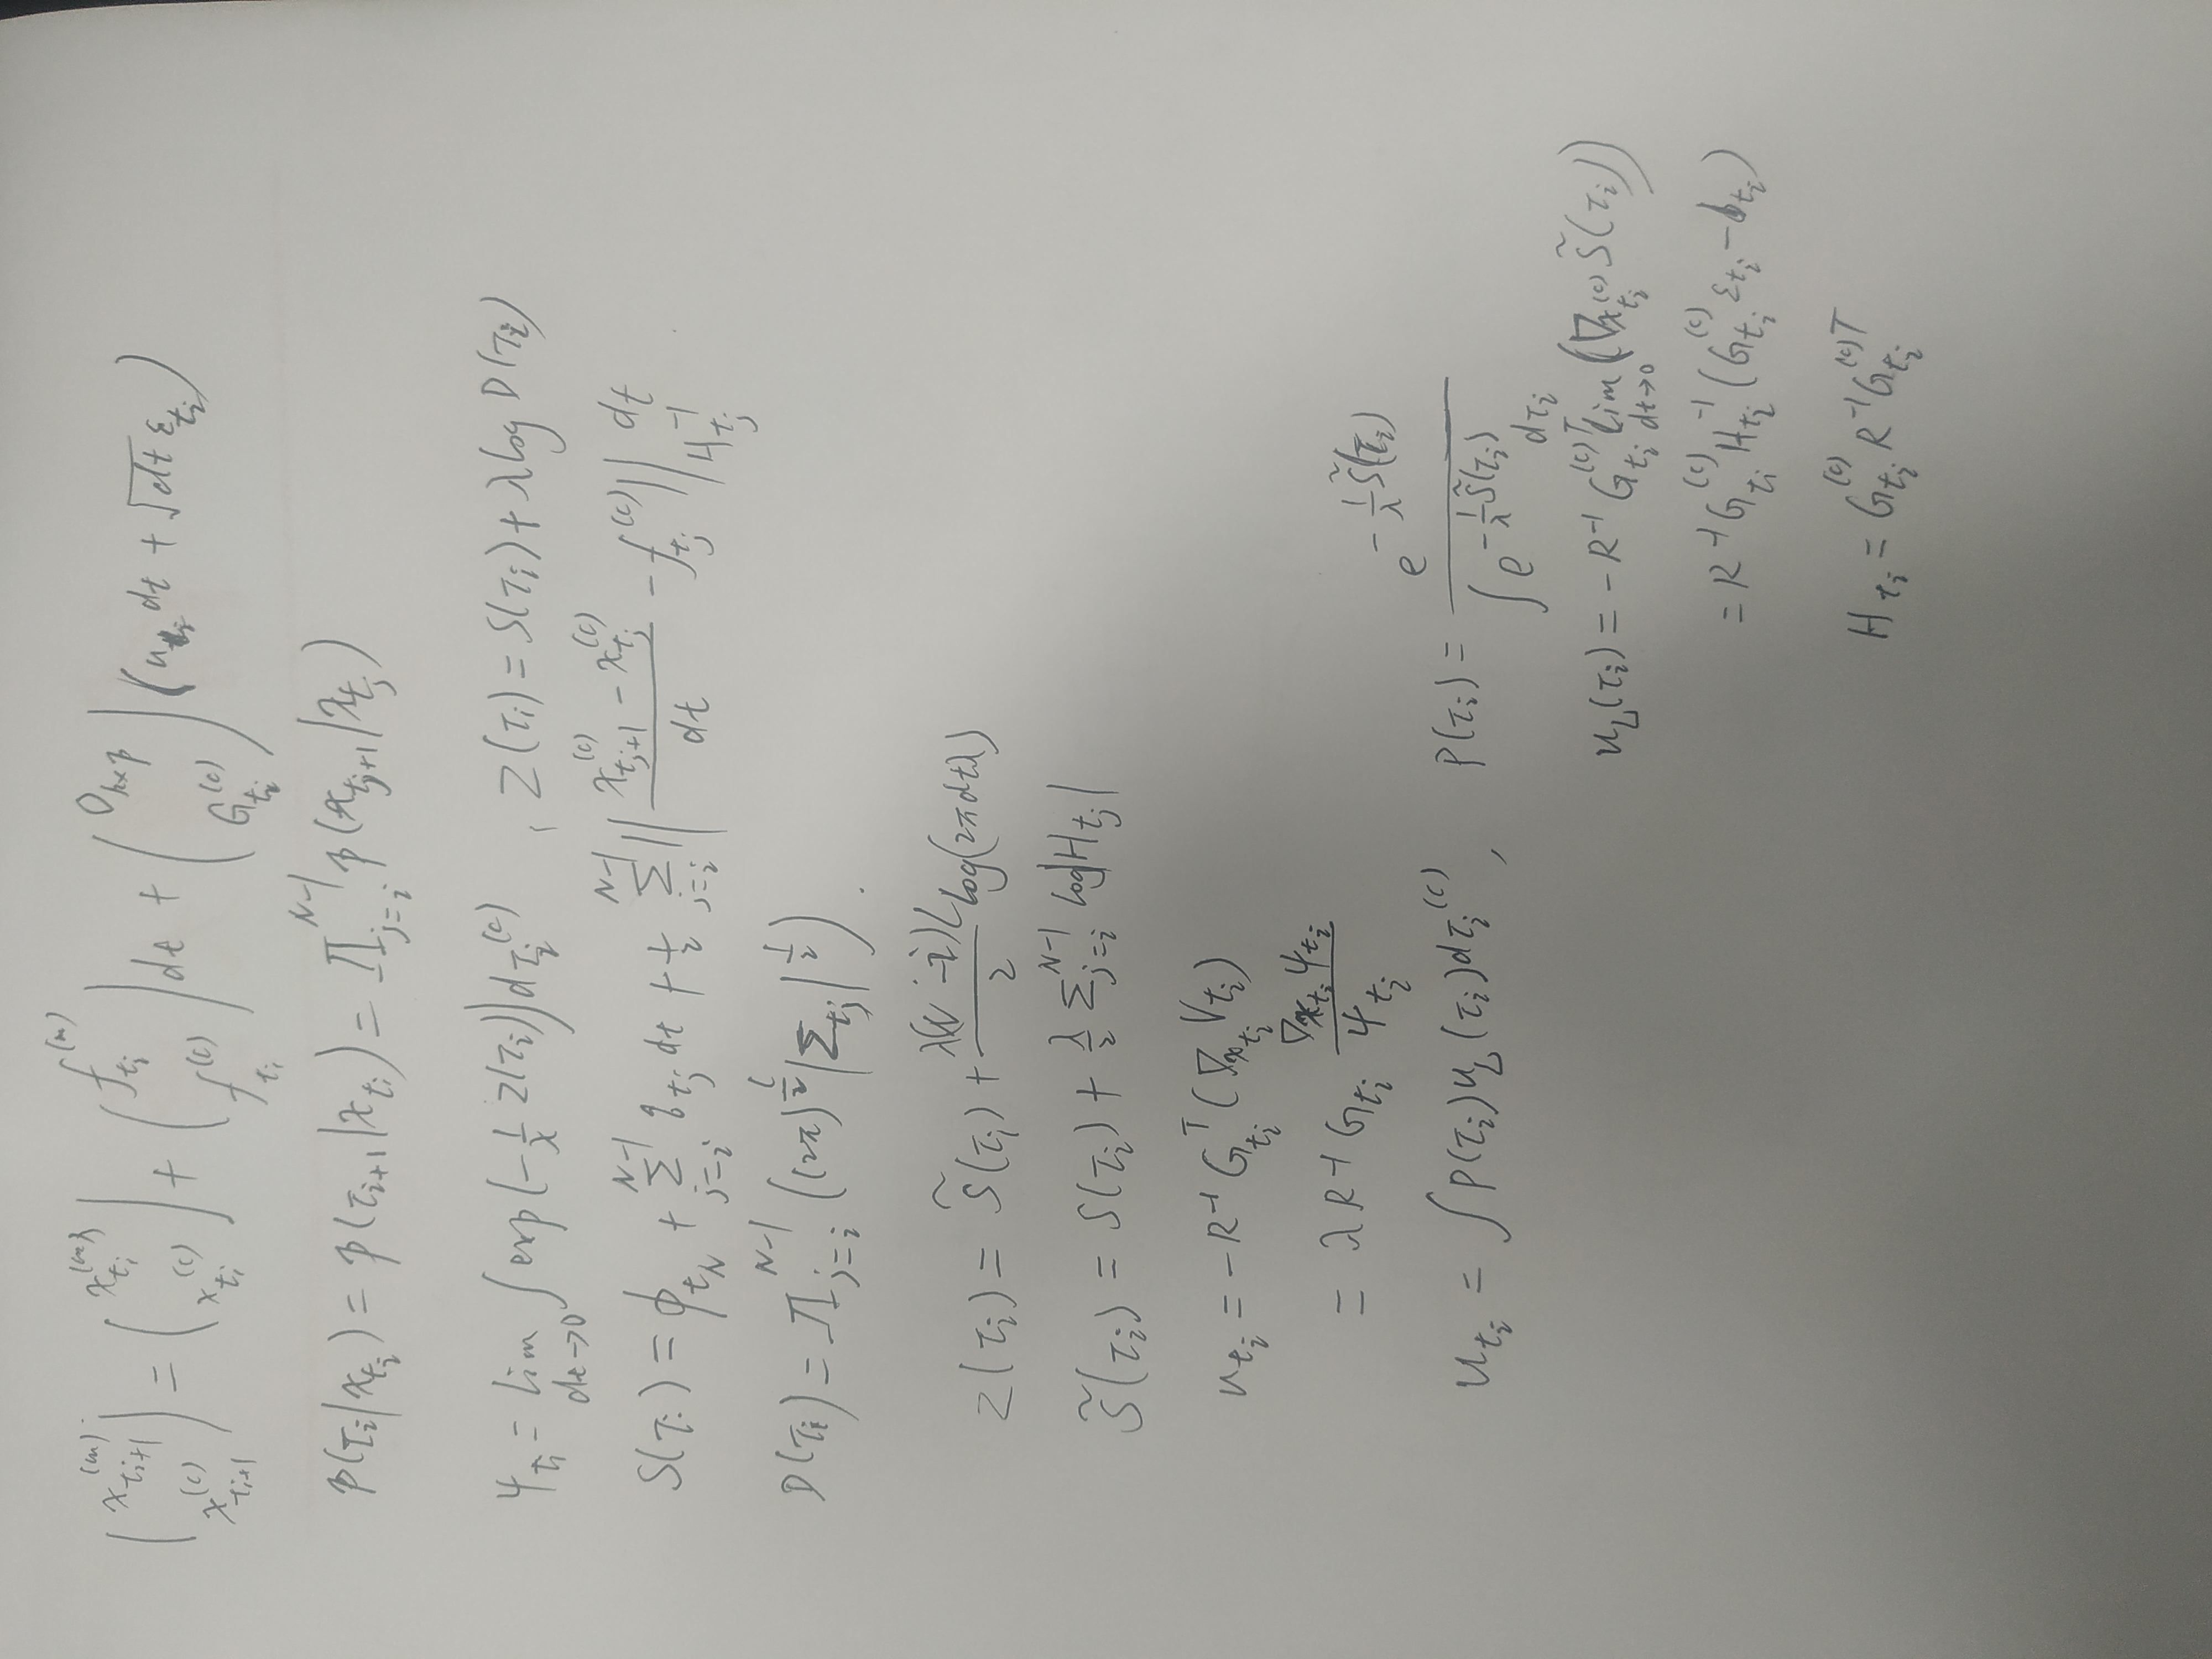
\includegraphics[height=18cm,angle=270]{1.jpg}}
  		   
    		\end{figure}



\end{document}